\newcommand{\nom}{Porte conteneur}
\newcommand{\sequence}{03}
\newcommand{\num}{04}
\newcommand{\type}{TD}
\newcommand{\descrip}{Résolution d'un problème en utilisant des méthodes algorithmiques}
\newcommand{\competences}{Alt-C3: Concevoir un algorithme répondant à un problème précisément posé}

\documentclass[10pt,a4paper]{article}
  \usepackage[french]{babel}
  \usepackage[utf8]{inputenc}
  \usepackage[T1]{fontenc}
  \usepackage{xcolor}
  \usepackage[]{graphicx}
  \usepackage{makeidx}
  \usepackage{textcomp}
  \usepackage{amsmath}
  \usepackage{amssymb}
  \usepackage{stmaryrd}
  \usepackage{fancyhdr}
  \usepackage{lettrine}
  \usepackage{calc}
  \usepackage{boxedminipage}
  \usepackage[french,onelanguage, boxruled,linesnumbered]{algorithm2e}
  \usepackage[colorlinks=false,pdftex]{hyperref}
  \usepackage{minted}
  \usepackage{url}
  %\usepackage[locale=FR]{siunitx}
  \usepackage{multicol}
  \makeindex

  %\graphicspath{{../Images/}}

  \renewcommand\listingscaption{Programme}

  %\renewcommand{\thechapter}{\Alph{chapter}}
  \renewcommand{\thesection}{\Roman{section}}
  %\newcommand{\inter}{\vspace{0.5cm}%
  %\noindent }
  %\newcommand{\unite}{\ \textrm}
  \newcommand{\ud}{\mathrm{d}}
  \newcommand{\vect}{\overrightarrow}
  %\newcommand{\ch}{\mathrm{ch}} % cosinus hyperbolique
  %\newcommand{\sh}{\mathrm{sh}} % sinus hyperbolique

  \textwidth 160mm
  \textheight 250mm
  \hoffset=-1.70cm
  \voffset=-1.5cm
  \parindent=0cm

  \pagestyle{fancy}
  \fancyhead[L]{\bfseries {\large PTSI -- Dorian}}
  \fancyhead[C]{\bfseries{{\type} \no \num}}
  \fancyhead[R]{\bfseries{\large Informatique}}
  \fancyfoot[C]{\thepage}
  \fancyfoot[L]{\footnotesize R. Costadoat, J. Genzmer, W. Robert}
  \fancyfoot[R]{\small \today}
  
  \definecolor{bg}{rgb}{0.5,0.5,0.5}
  \definecolor{danger}{RGB}{217,83,79}
  
  \fancypagestyle{correction}{%
  \fancyhf{}
  \lhead{\colorbox{danger}{\begin{minipage}{0.65\paperwidth} \textcolor{white}{\textbf{Correction}} \end{minipage}} }
  \rhead{
\includegraphics[width=2cm]{../../img/logo}}
  \lfoot{Juliette Genzmer, Willie Robert, Renaud Costadoat}
  \rfoot{\colorbox{danger}{\begin{minipage}{0.6\paperwidth} \begin{flushright}\textcolor{white}{\textbf{Correction}}\end{flushright} \end{minipage}} }}

  
  % macro Juliette
  
\usepackage{comment}   
\usepackage{amsthm}  
\theoremstyle{definition}
\newtheorem{exercice}{Exercice}
\newtheorem*{rappel}{Rappel}
\newtheorem*{remark}{Remarque}
\newtheorem*{defn}{Définition}
\newtheorem*{ppe}{Propriété}
\newtheorem{solution}{Solution}


\begin{document}

\section{Présentation du système}

\subsection{Contexte de l'étude}

\begin{minipage}{0.55\linewidth}
La nécessité de diminuer le coût de transport des marchandises embarquées sur les bateaux  porte-conteneurs impose de limiter au maximum le temps d'immobilisation des navires à quai. 

Un portique permet de transborder un ou plusieurs conteneurs d'un quai à un emplacement sur un bateau porte-conteneurs.
\end{minipage}
\hfill
\begin{minipage}{0.4\linewidth}
 \centering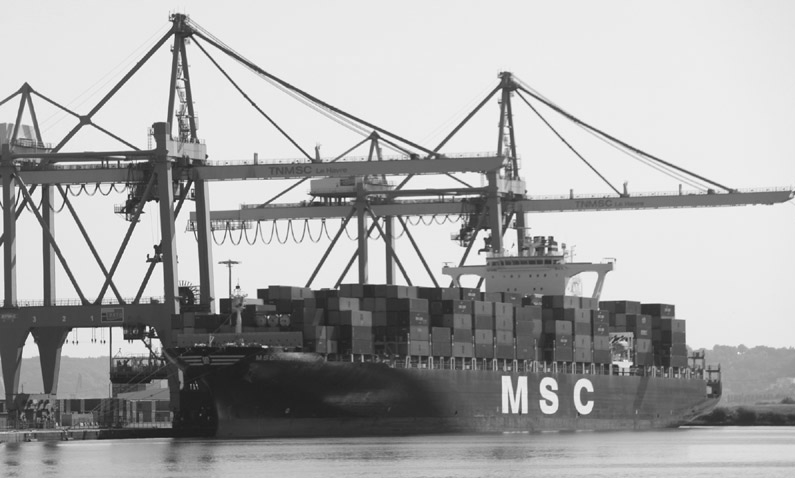
\includegraphics[width=0.9\linewidth]{img/fig1}
\end{minipage}

Le développement de portiques permettant de déplacer plusieurs conteneurs simultanément en un temps minimum permet des économies importantes pour les armateurs.

La société MSC a commandé la conception de trois portiques \og nouvelles générations \fg à l'entreprise chinoise ZMPC pour ses nouvelles installations de Port 2000 au Havre.
	
Un portique est constitué :
\begin{itemize}
 \item d'une structure acier qui se déplace le long de rails ancrés dans le béton du quai,
 \item d'un chariot porteur qui saisit un conteneur sur le quai pour le poser sur une plateforme intermédiaire arrimée à la structure,
 \item d'un chariot principal qui permet de déplacer un conteneur de la plate-forme intermédiaire jusqu'au bateau.
\end{itemize}

Chaque chariot est constitué d'une salle des machines et d'un spreader, bloc d'accroche des conteneurs, reliés par quatre câbles.

\begin{center}
 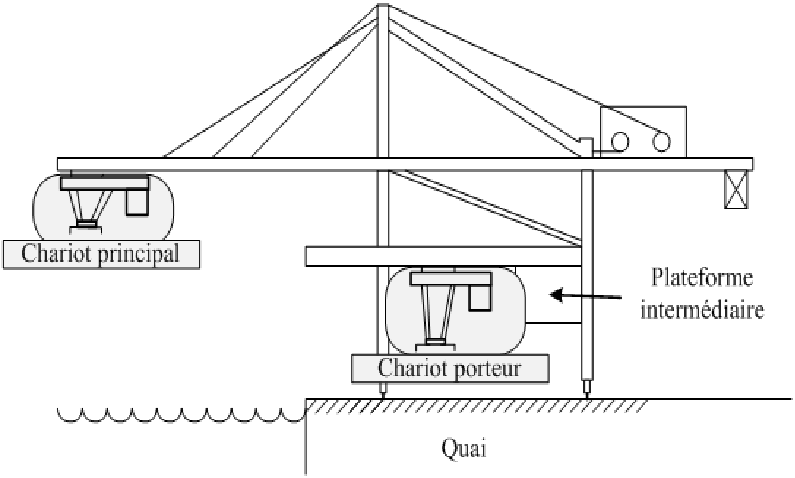
\includegraphics[width=0.5\linewidth]{img/fig2}
\end{center}

\begin{center}
 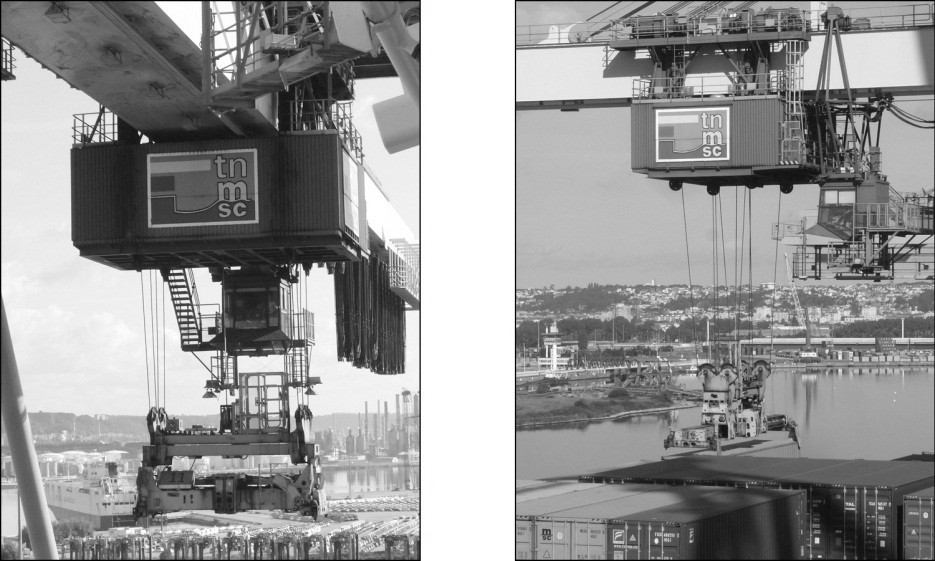
\includegraphics[width=0.5\linewidth]{img/fig3}
\end{center}


\section{Freiner et bloquer l'ensemble S = {spreader + conteneur} (1h30)}

L'objectif de cette partie est d'étudier le frein mécanique utilisé lors d'un arrêt de sécurité.

\subsection{Freinage mécanique}

\begin{minipage}{0.7\linewidth}
Le frein de service retenu par le concepteur est le frein Bubenzer SB28-Ed 301/10bb associé à un disque de diamètre 800 mm. Les caractéristiques des freins SB28 sont présentées sur le document technique DT6. Ce frein a la particularité d'associer une unité hydraulique à un frein à disque formant ainsi un ensemble autonome électrique.
\end{minipage}
\hfill
\begin{minipage}{0.27\linewidth}
 \centering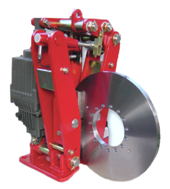
\includegraphics[width=0.9\linewidth]{img/fig17}
\end{minipage}

Hypothèses :
\begin{itemize}
 \item l'action de la pesanteur est négligée,
 \item les liaisons autres que les liaisons appuis plans sont supposées parfaites.
\end{itemize}

Le schéma cinématique de ce frein lorsque le disque de frein est en mouvement est présenté ci-dessous. L'effort de serrage $\overrightarrow{F}$ est exercé verticalement par des rondelles coniques lorsque l'alimentation électrique du frein est coupée. On prendra $\|\overrightarrow{F}\|=1kN$.

\begin{center}
 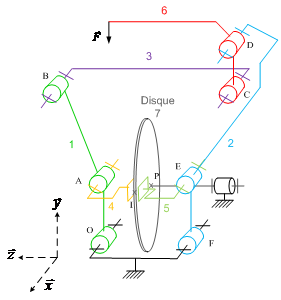
\includegraphics[width=0.4\linewidth]{img/fig18}
\end{center}

Une projection plane de ce schéma est donnée dans la suite avec les dimensions correspondantes. Le modèle a été modifié afin de simplifier la résolution de l'étude.

Les liaisons en A, B, C, D, E, F et O sont des liaisons pivot d'axe $\overrightarrow{x}$.

Le problème sera considéré comme plan $(\overrightarrow{y},\overrightarrow{z})$.
\\ ~\ \\
\begin{minipage}{0.65\linewidth}
 \centering 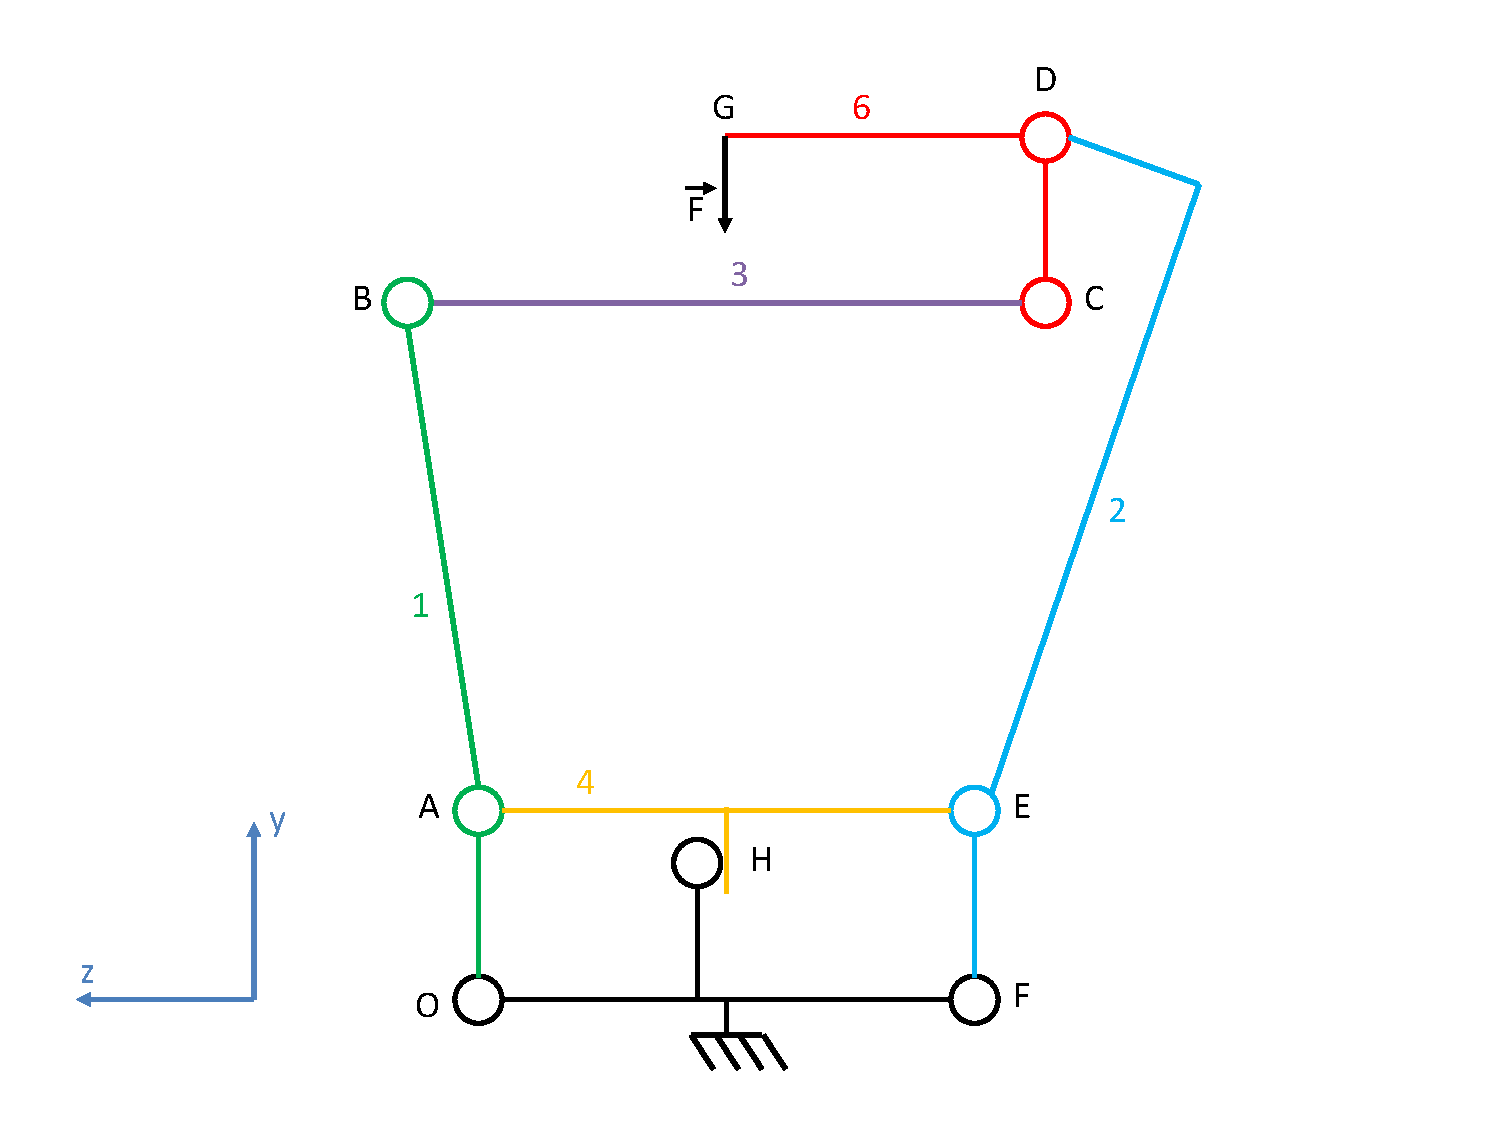
\includegraphics[width=1\linewidth]{img/Figure_stat_2}
\end{minipage}
\hfill
\begin{minipage}{0.3\linewidth}
\begin{itemize}
 \item $\overrightarrow{DG}=l_1.\overrightarrow{z}$,
 \item $\overrightarrow{CD}=l_2.\overrightarrow{y}$,
 \item $\overrightarrow{FE}=\overrightarrow{OA}=l_3.\overrightarrow{y}$,
 \item $\overrightarrow{EC}=l_4.\overrightarrow{y}-l_5.\overrightarrow{z}$,
 \item $\overrightarrow{AB}=l_4.\overrightarrow{y}+l_5.\overrightarrow{z}$,
 \item $\overrightarrow{FO}=l_6.\overrightarrow{z}$,
 \item $\overrightarrow{EA}=l_6.\overrightarrow{z}$,
 \item $\overrightarrow{EH}=\dfrac{l_6}{2}.\overrightarrow{z}$.
\end{itemize}
\end{minipage}

\begin{minipage}{0.45\linewidth}
Le résultat de l'étude statique correspond aux équations suivantes: \\
$\left\{\begin{array}{l}
Y_{13}-Y_{36}=0 \\ Z_{13}-Z_{36}=0 \\ -(2.l_5+l_6).Y_{13}=0 \\
-Y_{62}-F=0 \\ Z_{36}-Z_{62}=0 \\ -l_2.Z_{36}+l_1.F=0 \\
-Y_{41}-Y_{42}=0 \\ -Z_{41}-Z_{42}+Z_{04}=0 \\ l_6.Y_{41}=0 \\
Y_{02}+Y_{62}=0 \\ Z_{02}+Z_{42}+Z_{62}=0 \\ l_3.Z_{42}+(l_2+l_3+l_4).Z_{62}+l_5.Y_{62}=0 \\
Y_{01}=0 \\ Z_{41}-Z_{13}+Z_{01}=0 \\ l_3.Z_{41}-(l_3+l_4).Z_{13}=0 \end{array}\right.$
\end{minipage}
\hfill
\begin{minipage}{0.45\linewidth}
Distances (mm) et effort (N):
\begin{itemize}
 \item $l_1=200$,
 \item $l_2=100$,
 \item $l_3=100$,
 \item $l_4=350$,
 \item $l_5=50$,
 \item $l_6=400$,
 \item $F=2000N$.
\end{itemize}
\end{minipage}

\paragraph{Question 1:} Proposer une matrice $A$, un vecteur $Y$ et un vecteur $X$ (représentant les inconnues) afin de résoudre ce problème à l'aide du pivot de Gauss.

\paragraph{Question 2:} Coder la résolution de ce problème à l'aide de l'algorithme du pivot de Gauss.

\paragraph{Question 3:} Donner les valeurs solutions de ce système.

\ifdef{\public}{\end{document}}

\newpage

\pagestyle{correction}\setcounter{section}{0}

\paragraph{Question 1:}
 ~\ \\ ~\ \\
$X=\left(\begin{array}{c}
Y_{13} \\ Z_{13} \\ Y_{36} \\ Z_{36} \\ Y_{62} \\ Z_{62} \\
Y_{41} \\ Z_{41} \\ Y_{42} \\ Z_{42} \\ Z_{04} \\ Y_{02} \\
Z_{02} \\ Y_{01} \\ Z_{01}\end{array}\right)$
\\ ~\ \\ ~\ \\
Matrice A:\\ ~\ \\
$\left(\begin{array}{c c c c c c c c c c c c c c c}
1 & 0 & -1 & 0 & 0 & 0 & 0 & 0 & 0 & 0 & 0 & 0 & 0 & 0 & 0 \\
0 & 1 & 0 & -1 & 0 & 0 & 0 & 0 & 0 & 0 & 0 & 0 & 0 & 0 & 0 \\
-(2*l5+l6) & 0 & 0 & 0 & 0 & 0 & 0 & 0 & 0 & 0 & 0 & 0 & 0 & 0 & 0 \\
0 & 0 & 0 & 0 & -1 & 0 & 0 & 0 & 0 & 0 & 0 & 0 & 0 & 0 & 0 \\
0 & 0 & 0 & 1 & 0 & -1 & 0 & 0 & 0 & 0 & 0 & 0 & 0 & 0 & 0 \\
0 & 0 & 0 & -l2 & 0 & 0 & 0 & 0 & 0 & 0 & 0 & 0 & 0 & 0 & 0 \\
0 & 0 & 0 & 0 & 0 & 0 & -1 & 0 & -1 & 0 & 0 & 0 & 0 & 0 & 0 \\
0 & 0 & 0 & 0 & 0 & 0 & 0 & -1 & 0 & -1 & 1 & 0 & 0 & 0 & 0 \\
0 & 0 & 0 & 0 & 0 & 0 & l6 & 0 & 0 & 0 & 0 & 0 & 0 & 0 & 0 \\
0 & 0 & 0 & 0 & 1 & 0 & 0 & 0 & 0 & 0 & 0 & 1 & 0 & 0 & 0 \\
0 & 0 & 0 & 0 & 0 & 1 & 0 & 0 & 0 & 1 & 0 & 0 & 1 & 0 & 0 \\
0 & 0 & 0 & 0 & l5 & l2+l3+l4 & 0 & 0 & 0 & l3 & 0 & 0 & 0 & 0 & 0 \\
0 & 0 & 0 & 0 & 0 & 0 & 0 & 0 & 0 & 0 & 0 & 0 & 0 & 1 & 0 \\
0 & -1 & 0 & 0 & 0 & 0 & 0 & 1 & 0 & 0 & 0 & 0 & 0 & 0 & 1 \\
0 & -(l3+l4) & 0 & 0 & 0 & 0 & 0 & l3 & 0 & 0 & 0 & 0 & 0 & 0 & 0
\end{array}\right)$

$Y=\left(\begin{array}{c}
0 \\ 0 \\ 0 \\ F \\ 0 \\ -l1*F \\ 0 \\ 0 \\ 0 \\ 0 \\ 0 \\ 0 \\ 0 \\ 0 \\ 0\end{array}\right)$

\paragraph{Question 2:} Cf code Python

\paragraph{Question 3:} 
 ~\ \\ ~\ \\
$X=\left(\begin{array}{c}
0.0 \\ 3999.9999999999964 \\ -0.0 \\ 3999.9999999999964 \\  -2000.0 \\ 3999.9999999999964 \\ -0.0 \\ 17999.99999999999 \\ -0.0 \\ -20999.999999999993 \\ -3000.0000000000036 \\ 2000.0 \\  16999.999999999996 \\ 0.0 \\ -13999.999999999993\end{array}\right)=\left(\begin{array}{c}
Y_{13} \\ Z_{13} \\ Y_{36} \\ Z_{36} \\ Y_{62} \\ Z_{62} \\
Y_{41} \\ Z_{41} \\ Y_{42} \\ Z_{42} \\ Z_{04} \\ Y_{02} \\
Z_{02} \\ Y_{01} \\ Z_{01}\end{array}\right)=\left(\begin{array}{c}
0. \\ 4000. \\ -0. \\ 4000. \\ -2000. \\ 4000. \\ -0. \\
18000. \\ -0. \\ -21000. \\ -3000. \\ 2000. \\ 17000. \\ 0. \\ -14000.\end{array}\right)$

\end{document}
